\section{Experiments: Scaffolding Feedback}
Following our deployments, we conducted two empirical studies to investigate the impact of suggestions and guidance on feedback quality.

\subsection{EXP 1: Do Static Suggestions Improve Feedback?}
In an online between-subjects study, 40 undergraduate design students were asked to review three restaurant website homepages using CritiqueKit. The task emulated peer review tasks often required in creative courses. This study's suggestion corpus came from a design feedback task on CrowdCrit [25] and was categorized in the Positive, Problem, and Solution categories. We hypothesized that suggestions and guidance would help reviewers provide more specific and actionable comments.

\begin{figure}
\centering
  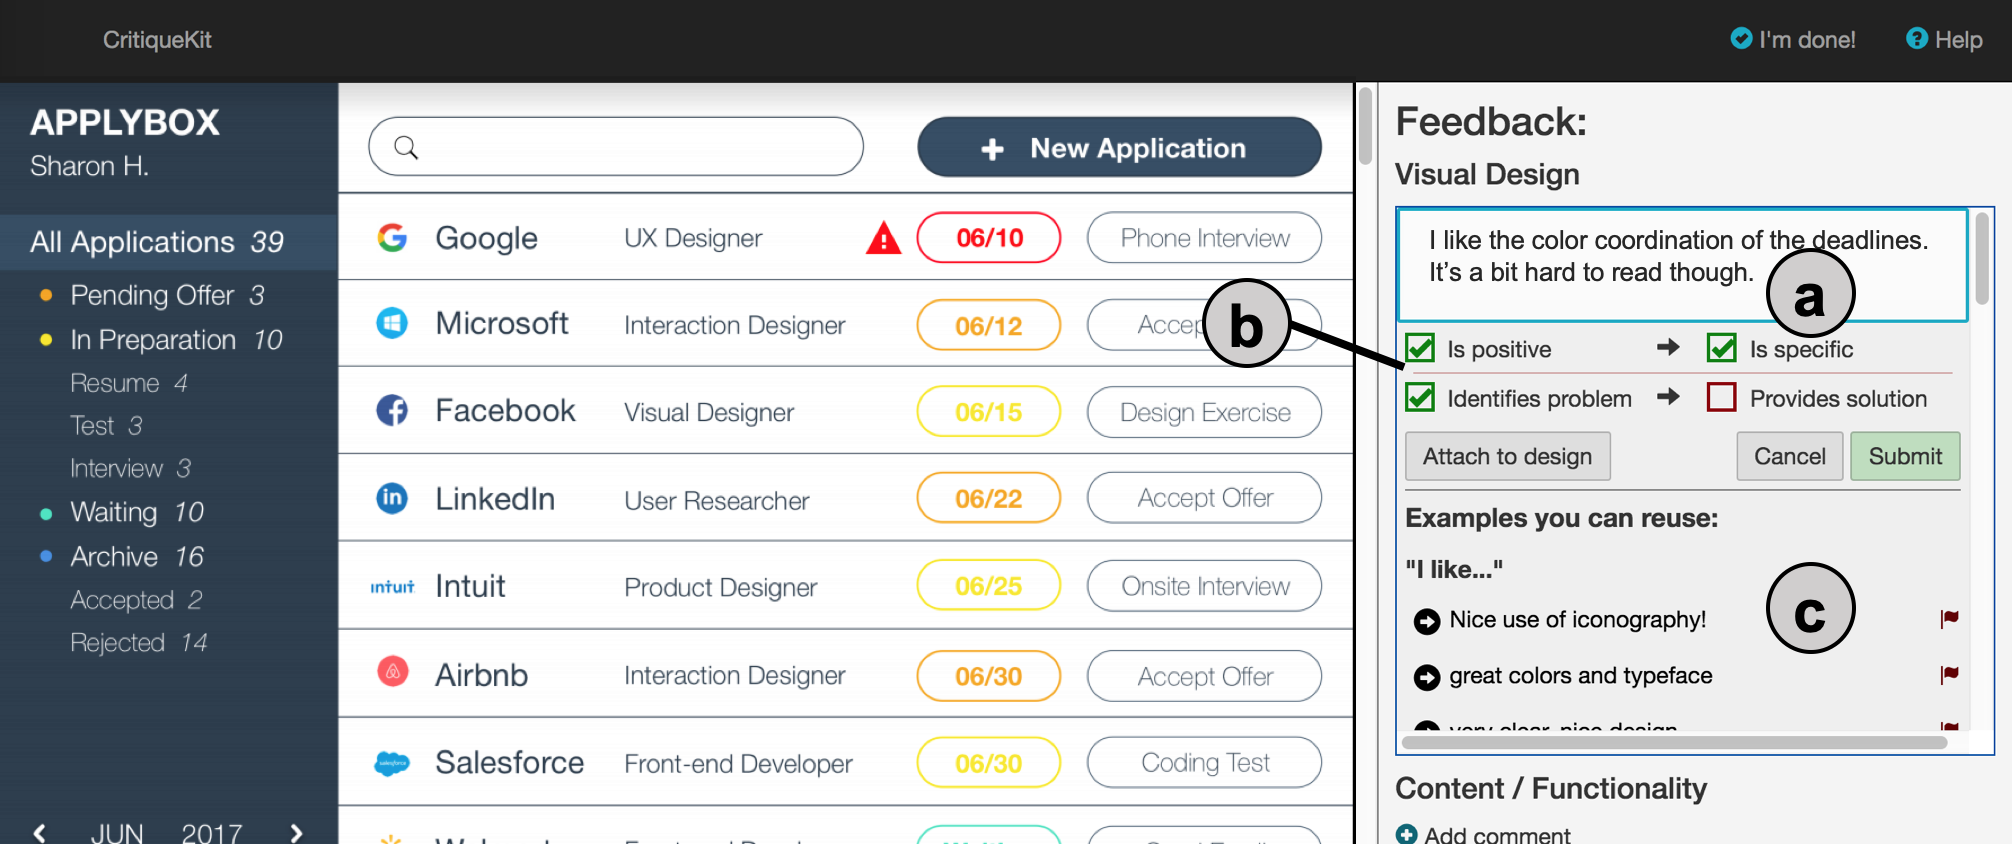
\includegraphics[width=\textwidth]{critiquekit/figures/old_interface.png}
  \caption{The CritiqueKit user interface for EXP 1. a) The reviewer types their feedback into the text box. b) Checkboxes in the guidance panel update as the reviewer types to show how well the comment fulfills high-quality feedback criteria. c) The reviewer can browse and reuse previously given feedback.}~\label{fig:critiquekit_exp1}
\end{figure}

\subsubsection{Method: Reviewing Restaurant Websites}
40 participants were randomly assigned to either the CritiqueKit condition or the Control condition (20 in each). CritiqueKit participants used the same version of CritiqueKit as DEP 2 with all features available (\autoref{fig:critiquekit_exp1}). Control participants used an otherwise identical version consisting solely of a comment text box. Upon landing on the homepage of either version, participants were provided with a scenario explaining that three restaurant owners are seeking feedback on their new website design. Participants were given a brief tutorial of CritiqueKit's features and an explanation of what makes for good feedback. There were no restrictions or requirements on time spent or amount of feedback to provide. We compared the percentages of comments in five categories. Comments including a supportive element were labeled as \textit{Positive Only} or \textit{Positive + Specific}. Comments including a critical element were labeled \textit{Problem Only}, \textit{Solution Only}, or \textit{Problem + Solution}.

\begin{figure}
\centering
  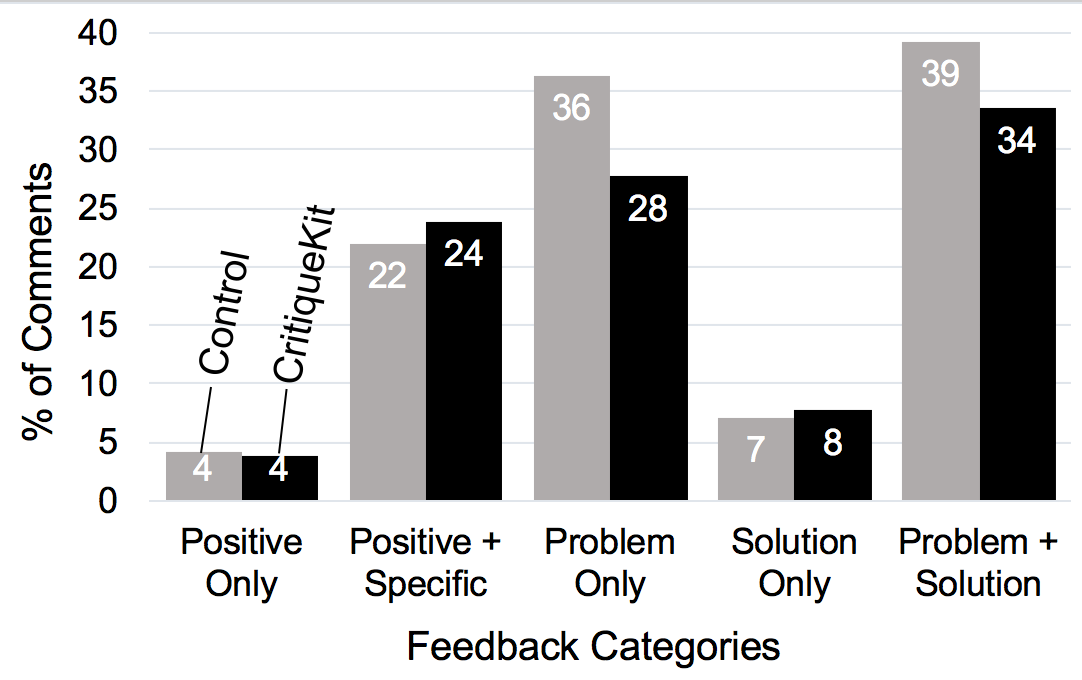
\includegraphics[width=0.6\textwidth]{critiquekit/figures/exp1_feedbacktypes.png}
  \caption{A plurality of feedback in both conditions in EXP 1 identified both a problem and solution (\textit{i.e.}, was actionable). Feedback that was only positive was the rarest. There were no significant differences between conditions for these categories.}~\label{fig:critiquekit_exp1_results}
\end{figure}

\subsubsection{Results: Static Suggestions Were Not Helpful}
With static suggestions and interactive guidance, there were no significant differences between conditions. (To foreshadow, we will see differences in EXP 2, which adds adaptive suggestions). Participants provided a total of 323 comments (168 for control, 155 for CritiqueKit). The average number of words per comment was not significantly different between conditions (Control: $m = 29.07, SD = 23.64$; CritiqueKit: $m = 23.22, SD = 17.3$) ($F(1,38) = 2.52, p = .11$).

\subsubsection{Suggestions \& Guidance Did Not Affect Type of Feedback}
The distribution of the five category types did not vary significantly between conditions ($x^2 = 4.80, df = 4, p = .31$) (\autoref{fig:critiquekit_exp1_results}). In both groups, participants provided mostly Problem + Solution feedback (39\% in Control; 34\% in CritiqueKit). 

\subsubsection{Most CritiqueKit Participants Corrected Category Labels}
65\% of CritiqueKit participants actively used the guidance panel, making a total of 85 corrections to categories. Interaction with the guidance panel may have indicated attention to the feedback characteristics. As the study was online, we don't know how many of the other 35\% were influenced by the guidance panel. 

\subsubsection{Unfortunately, People also Reused Vague Suggestions}
11 distinct suggestions from the corpus were reused. 8 of these were vague; 3 were specific. 15 of 155 reviews included a reused suggestion. This seems especially low given the high engagement with the guidance panel. We see two reasons for this: First, the suggestions came from CrowdCrit [25], where participants provided feedback on a weather app design. The study task was different than the task for which the suggested feedback was originally given, and novices may have had a limited ability to see the deep structure behind a suggestion and reapply it in a new context. Second, the suggestions were created by crowd workers and of uneven quality. 

The suggestions selected were typically short, positive comments, perhaps because students did not know how to apply them in the specific context. For example, the most commonly reused suggestion was ``great use of color'' (reused 3 times). This result is similar to DEP2 in which students did not find feedback provided by other peers or novices to be useful and generalizable. Feedback suggestions may require more curation or quality control to be most useful. 

\subsubsection{Suggestions \& Guidance Should Work in Concert}
While this version of CritiqueKit contained both feedback suggestions and interactive guidance, these features functioned independently. Regardless of the categories checked in the guidance panel, the suggestions remained static and presented in the same order for each participant, potentially making them easy to ignore if they were irrelevant to the context. Participants may have paid attention to only one feature at a time. The next study investigated the question of whether adaptively presenting feedback suggestions along with interactive guidance improves feedback. 

\subsection{EXP 2: Do Adaptive Suggestions Help?}
The second experiment used the final version of CritiqueKit described in the system section to test the hypothesis that adaptively-presented suggestions combined with guidance would improve feedback by increasing the fraction of feedback that is specific, actionable, and/or justified.

\subsubsection{Method: Reviewing Paper Prototypes}
We conducted a between-subjects in-person study with 47 (27 female) participants. Participants were recruited from an undergraduate subject pool within the Psychology and Cognitive Science departments. Participants were randomly assigned to either the CritiqueKit ($n = 24$) or Control ($n = 23$) conditions. 44 of these participants had no design course experience; 3 participants had taken at least one design course. 28 spoke English as a second language. 

Participants were asked to provide feedback on two designs from students enrolled in an online course who volunteered to receive more feedback on their work. These designs were PDFs of mobile application paper prototypes. The review criteria included whether the prototype supported the student's point of view and whether it seemed easily navigable. Participants were first shown the design instructions and review criteria and then given a short tutorial of CritiqueKit as well as an explanation of what makes for good feedback. CritiqueKit participants had all features of CritiqueKit available to them (\autoref{fig:critiquekit_interface}), while Control participants used a version that consisted of only a textbox for their feedback. The task took about 30 minutes to complete. After providing feedback on both designs, participants were interviewed about their feedback process and use of CritiqueKit. 

\subsubsection{Presenting Feedback Suggestions Adaptively}
The categories on the guidance panel and their definition used for coding participants' responses were the following:\\
\textbf{Specific}: relates directly to the review criteria\\
\textbf{Actionable}: gives a concrete suggestion for improvement\\
\textbf{Justified}: provides a reason for why something is done well or should be improved

For DEP 2 and EXP 1, the guidance panel categories sought to encourage specific and actionable feedback (\autoref{fig:critiquekit_exp1}). Examining the feedback from our previous studies, we found that ``Is Positive'' and ``Identifies a Problem'' did not provide significant guidance as reviewers were generally aware of whether their feedback was positive or critical. In addition, the guidance panel did not explicitly check for justification of feedback. For EXP 2, we revised the categories to ``Is Specific,'' ``Is Actionable,'' and ``Is Justified'' to also encourage the explanation or reasoning behind feedback. As described in the system section, the checkboxes update as the reviewer types to reflect the categories present in their comment, and the suggestions adapt to show feedback examples from categories not yet present in the comment. 

\begin{figure}
\centering
  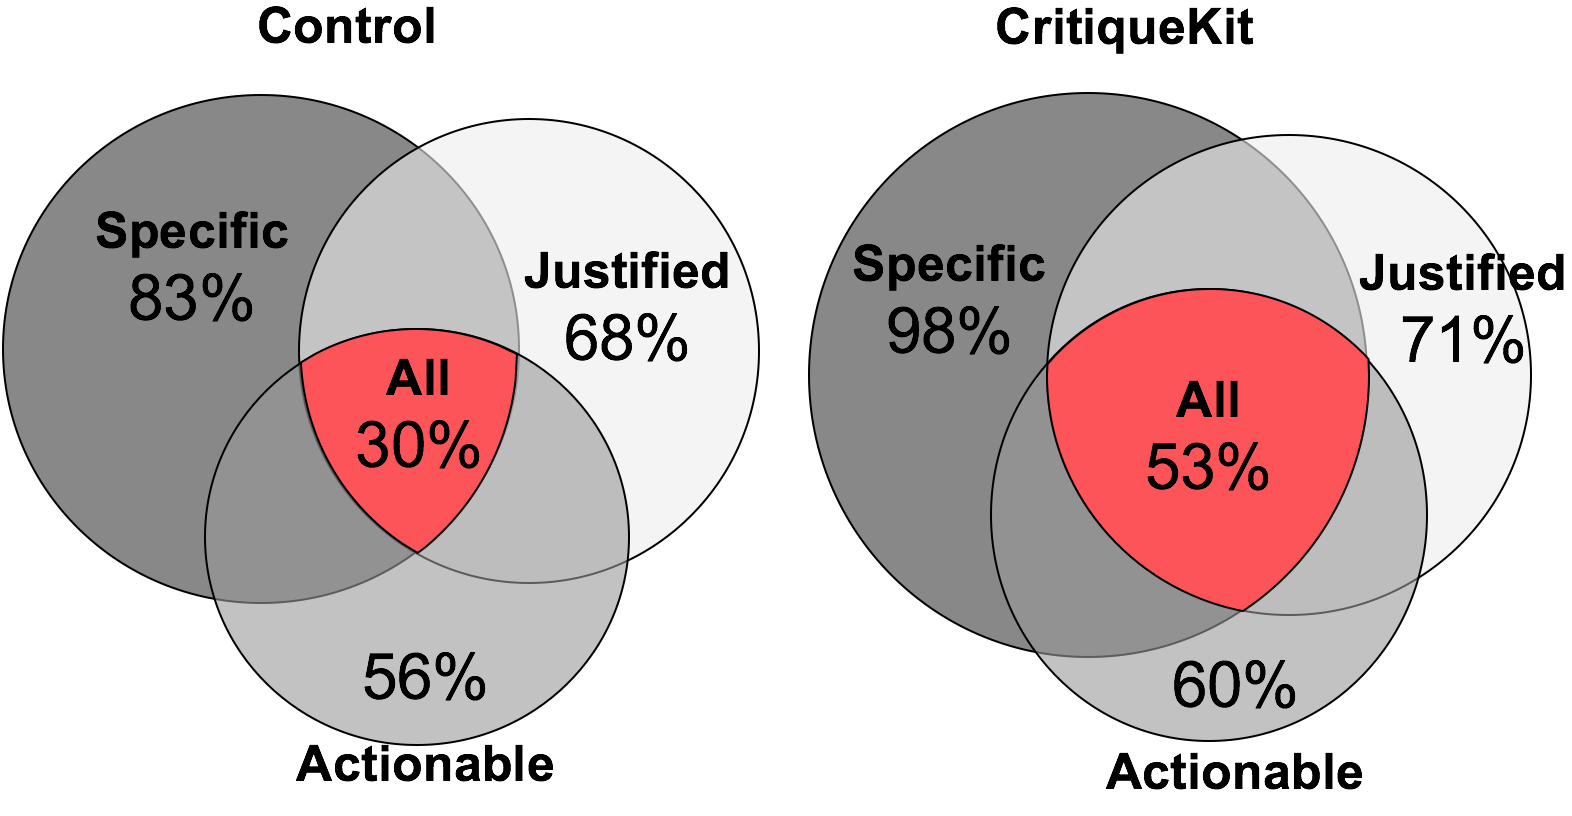
\includegraphics[width=0.6\textwidth]{critiquekit/figures/venn_diagram_exp2.png}
  \caption{In a controlled experiment, a significantly higher percentage of feedback in the CritiqueKit condition (53\% versus 30\%) contained three attributes of good feedback: Specific, Actionable, and Justified.}~\label{fig:critiquekit_exp2}
\end{figure}

\subsubsection{Results: CritiqueKit Participants Provided More Specific, Actionable, \& Justified Feedback}
Participants provided 158 total comments (79 control, 79 CritiqueKit). The percentage of comments that contained all three categories (specific, actionable, and justified) was significantly higher in the CritiqueKit condition (53\%) than in Control (30\%) ($x^2=8.33, df = 1, p = .01$) (\autoref{fig:critiquekit_exp2}). As an example, this comment meets all three: ``The `more questionnaires' section (Specific) should be made smaller (Actionable) because it is not the main focus of the page.'' (Justified). The system's heuristic for checking specificity of a comment was quite simple: five words or greater in length. Feedback raters blind to each condition used a more sophisticated and holistic assessment, taking specific to also mean related to the review criteria. With this assessment, 98\% of CritiqueKit comments were labeled by raters as specific whereas only 83\% of Control comments were. These raters also rated comments from EXP 1 within the specific, actionable, and justified categories to provide a comparison between the two experiments. Interestingly, the percentage of comments containing all attributes in the Control condition was relatively consistent between EXP 1 (35\%) and EXP 2 (30\%). The percentage of comments with all attributes in the CritiqueKit condition greatly increased between the two experiments (26\% versus 53\%). Having the checkboxes may have explicitly reminded CritiqueKit participants to ensure their comments satisfy the specific, actionable, and justified categories.

\begin{figure}
\centering
  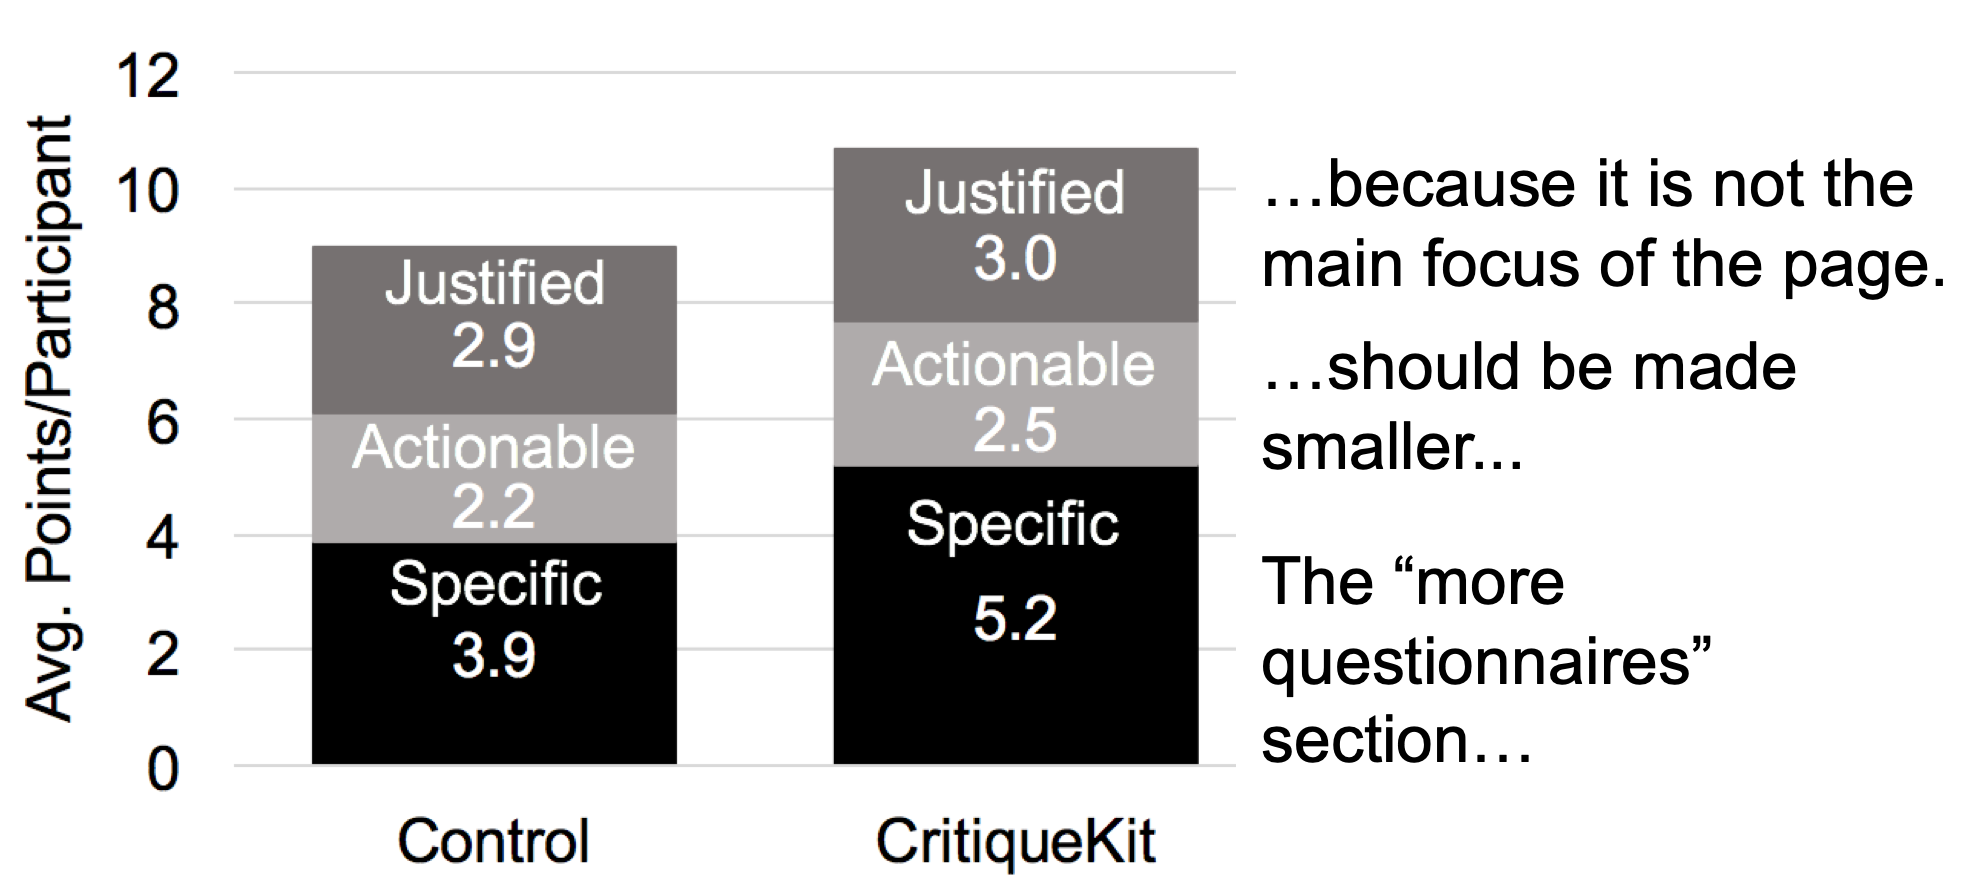
\includegraphics[width=0.6\textwidth]{critiquekit/figures/exp2_bar.png}
  \caption{CritiqueKit participants provided more \textit{specific} and \textit{all-three} category ideas than control participants.}~\label{fig:critiquekit_exp2_bar}
\end{figure}

Because longer comments were more likely to contain all three categories, each comment was also scored on a point scale and averaged per participant. Comments received one point for each specific, actionable, and justified idea (\autoref{fig:critiquekit_exp2_bar}). A \textsc{manova} with category points as dependent variables shows a significant difference between conditions ($F(1,3) = 3.21, p < .005$). CritiqueKit participants provided more specific ideas than Control participants (Control $m = 3.87$, CritiqueKit $m = 5.17$, $F(1,156) = 14.04, p  <  .05$). This may be because the suggestions provided examples of relevant ideas and led CritiqueKit participants to address more. CritiqueKit participants also provided more ideas that fit all three categories than control (Control $m = 1.0$, CritiqueKit $m = 2.2$, $F(1,156) = 8.78, p < .005$). Given that most participants did not have any design experience, the combination of adaptive suggestions and guidance may have been most useful for these reviewers. The suggestions may have provided a starting point while the guidance panel helped them understand how to apply the attributes of good feedback. There were no significant differences in the average number of actionable and justified ideas in comments.

On average, Control comments were 39.3 ($SD = 30.3$) words long and 43.7 ($SD = 31.4$) words for CritiqueKit comments. There was no significant difference in comment length ($F(1,156) = 1.77, p = .19$). Unfortunately, we don't know how the feedback improved students' work because they received feedback from both Control and CritiqueKit participants. A longitudinal deployment with the final version of CritiqueKit would likely be more useful in determining the helpfulness of feedback.

\subsubsection{Suggestions Helped Reviewers Describe Their Thoughts}
Participants rated the suggestions as being generally helpful ($m = 4.29, SD = 0.95$, 1-5 Likert Scale). When asked to elaborate on their rating, many participants noted that the suggestions helped them describe their thoughts. One participant remarked, ``\textit{I was a bit lost at first because I didn't know how to describe my thoughts. The suggestions helped me figure out how I should describe what I was thinking}.'' Similarly, another mentioned that ``\textit{when I [didn't] know how to put my feedback in words, I could look at the suggestions}.'' Particularly for participants without any design experience, suggestions helped with appropriate language to use in their feedback. For example, one noted that ``\textit{seeing actual wording from a designer's point of view was good so you know how to say what you want to say}.'' Though a few participants did not directly select suggestions, it is likely that they were inspired or influenced by them as they used similar wording in their own comments. 

Still, some participants felt the suggestions were too general and not entirely relevant to the specific design they were reviewing. One participant felt constrained by the suggestions, stating that she ignored them because she wanted to write her own opinions. Suggestions seemed most helpful for participants who used them as a starting point for their own thoughts rather than solely relying on them. Participants who simply selected suggestions tended to list issues without adding their own elaboration. This behavior not only led to incomplete feedback, but also produced depersonalized and scattered comments. For example, one comment that solely relied on suggestions reads ``User immediately knows the purpose of the prototype. Good use of grid layout to keep items aligned. Icons should be immediately recognizable to the user.'' A consideration for future work is to develop feedback suggestions tailored to help reviewers provide more cohesive and contextual comments. 

Most participants in this experiment did not have any design experience and may have benefited most from the suggestions. Many participants noted using the suggestions as a way to find ideas whereas students with design experience may already have heuristics and processes in mind when providing feedback. Future work should examine how suggestions and guidance might improve feedback for more experienced learners as well.

\subsubsection{Interactive Guidance Helped Remind \& Focus Reviewers} 
Participants were mixed on the helpfulness of the guidance panel ($m = 3.67, SD = 1.2$, 1-5 Likert Scale). Those who did find it helpful noted that the categories helped guide their feedback process. For instance, one participant noted that he ``\textit{went in order of the checkboxes. First, I provided something specific, then something actionable, then justified it}.'' Another noted that the categories helped her know whether her feedback was actually useful or helpful, and one noted that the guidance panel ``\textit{[made] sure the feedback is complete and not vague}.'' 

Anecdotally, we observed that when participants said the categories were not useful, it was because they believed them to be inaccurate in their classifications. The accuracy (compared to human raters) for the actionable category was 67\% and 75\% for the justified category. A participant stated that ``\textit{[the checkboxes] didn't always check when I thought they should, so I would just do it myself}.'' Another thought the checkboxes were ``\textit{quick to judge, it felt like it wasn't reading what I was saying}.'' Three participants, who were not native English speakers, found the categories confusing because they weren't sure what they meant. Future iterations of CritiqueKit could include the definition of these categories in the prompts to make the meaning clearer. Interestingly, a couple participants noted that they used the categories as reminders rather than for active guidance. For instance, a participant mentioned that though he felt the interactive guidance was not that accurate, ``\textit{[the checkboxes] reminded me to make sure my comment contained specific, actionable, and justified parts, so I'd go and reread through my comment}.'' 

Some participants commented on the adaptive presentation of the suggestions with the guidance panel. For one participant, the suggestions helped him understand what the categories meant. He noted, ``\textit{The whole actionable and justified thing, I didn't know what that meant, so the suggestions helped with that}.'' Observations of participants showed that some clicked on the checkboxes simply to see the suggestions under each one. When asked about how useful they found CritiqueKit in general, participants varied widely in their ratings of usefulness. A more precise measure would allow participants to compare across conditions, which was not possible with this between-subjects design. 
